\documentclass[11pt,a4paper]{article}
\usepackage[T1]{fontenc}
\usepackage{lmodern}
\usepackage{microtype}
\usepackage[margin=2.6cm]{geometry}
\usepackage{amsmath,amssymb,amsthm}
\usepackage{booktabs}
\usepackage{tikz}
\usepackage[hidelinks]{hyperref}
\usepackage{caption}

\newtheorem{proposition}{Proposition}

\definecolor{blue}{HTML}{2E6FBA}
\definecolor{red}{HTML}{C0392B}
\definecolor{stoneb}{HTML}{DCE8F6}
\definecolor{stoner}{HTML}{F6DCD9}

% \spikes{count}{colour}: a row of up to 5 spikes on the top side of a unit stone.
\newcommand{\spikes}[2]{%
  \ifnum#1>0
    \pgfmathsetmacro{\sw}{#1<=3 ? 0.18 : (#1==4 ? 0.145 : 0.12)}%
    \pgfmathsetmacro{\hw}{#1<=3 ? 0.075 : \sw/2}%
    \foreach \j in {1,...,#1}{%
      \pgfmathsetmacro{\sx}{(\j-(#1+1)/2)*\sw}%
      \fill[#2] (\sx-\hw,0.5) -- (\sx,0.66) -- (\sx+\hw,0.5) -- cycle;}%
  \fi}
% \stone{x}{y}{top}{right}{bottom}{left}{colour}{fill}{label}
\newcommand{\stone}[9]{\begin{scope}[shift={(#1,#2)}, scale=0.74]
  \filldraw[fill=#8, draw=#7, thick, rounded corners=1.5pt] (-0.5,-0.5) rectangle (0.5,0.5);
  \begin{scope}[rotate=0]\spikes{#3}{#7}\end{scope}
  \begin{scope}[rotate=-90]\spikes{#4}{#7}\end{scope}
  \begin{scope}[rotate=180]\spikes{#5}{#7}\end{scope}
  \begin{scope}[rotate=90]\spikes{#6}{#7}\end{scope}
  \node[font=\scriptsize\bfseries, text=#7] at (0,0) {#9};
\end{scope}}

\title{Chain Stones: rules, chains and the balance of a twenty-match run}
\author{Louis Vandenbruwaene}
\date{October 2026}

\begin{document}
\maketitle

\begin{abstract}
\noindent
Chain Stones is a placement game on a $4\times4$ board. Each stone is one of the six chess pieces, drawn as a character, with a fixed pattern of spikes on its four sides and a level from 1 to 5 that sets the number of spikes. A new stone fights its enemy neighbours, and then stones of different colours that touch across a spike keep fighting, closest to the new stone first, with every spike used up when it hits. The game is played as a run of twenty matches against seven computer opponents with fixed hidden decks. We show that every move ends, that afterwards no two stones of different colours touch across a spike, and that draws are possible. We describe how the opponents' decks were set by simulation and report $1{,}900$ simulated games with the final decks. A reference player who takes a level after every win wins $91\%$ of early matches, $74\%$ of middle ones, $44\%$ of late ones and $13\%$ against the final opponent, and clears a whole run about once in $18{,}000$ attempts. An appendix summarises the exact solution of the first version of the game on a $3\times3$ board.
\end{abstract}

\section{The game}

Chain Stones is played on a $4\times4$ board by two players, Blue (the human) and Red (the computer). Each holds a hand of eight stones. Red's hand is hidden from Blue until a stone is played. The players alternate placing one stone on an empty square, so after sixteen moves the board is full and both hands are empty.

\paragraph{Stones.} A stone is a piece and a level $\ell\in\{1,\dots,5\}$. Each chess piece has a base pattern of spikes on its four sides (top, right, bottom, left), and at level $\ell$ every side that has spikes in the base pattern gets $\ell-1$ more, up to $5$. The pawn and the knight come in four variants, each turned a quarter further, and every variant has its own name. Blue's stones face up the board and Red's stones are turned half way round. Table~\ref{tab:pieces} lists the chess pieces and figure~\ref{fig:pieces} draws them.

\begin{table}[ht]
\centering
\begin{tabular}{llll}
\toprule
code & chess piece & name & base (top, right, bottom, left) \\
\midrule
P & pawn & Tiny Tim, Tony, Tom, Ted & $(1,0,0,0)$, four turns \\
N & knight & Sir Gallops, Trots, Canters, Prances & $(2,0,0,2)$, four turns \\
B & bishop & Mitre Mandy & $(2,0,2,0)$ \\
R & rook & Castle Carl & $(0,2,0,2)$ \\
Q & queen & Her Majesty Mayhem & $(2,2,2,2)$ \\
K & king & Old King Coal & golden shields \\
\bottomrule
\end{tabular}
\caption{The chess pieces at level 1, facing up. Codes are used to write decks: R2 is Castle Carl at level 2 with spikes $(0,3,0,3)$, and a turned pawn or knight carries its direction, for example P1> for Tiny Tony with his spike to the right.}
\label{tab:pieces}
\end{table}

\begin{figure}[ht]
\centering
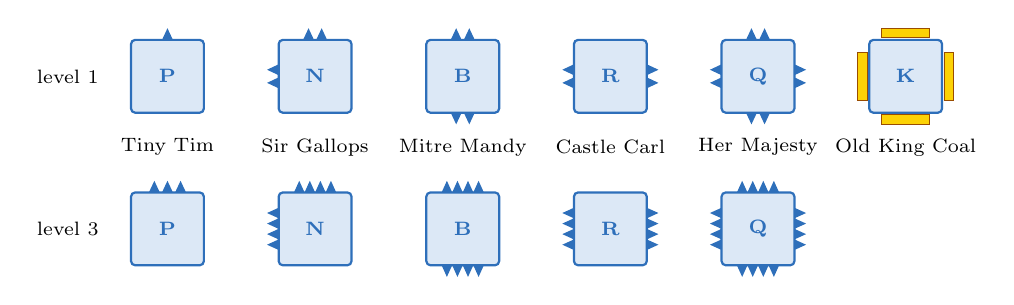
\begin{tikzpicture}[scale=1.25]
  \foreach \x/\t/\r/\b/\l/\n/\c in {0/1/0/0/0/P/Tiny Tim,1.5/2/0/0/2/N/Sir Gallops,3.0/2/0/2/0/B/Mitre Mandy,4.5/0/2/0/2/R/Castle Carl,6.0/2/2/2/2/Q/Her Majesty}{
    \stone{\x}{0}{\t}{\r}{\b}{\l}{blue}{stoneb}{\n}
    \node[font=\scriptsize] at (\x,-0.72) {\c};
  }
  \foreach \x/\t/\r/\b/\l/\n in {0/3/0/0/0/P,1.5/4/0/0/4/N,3.0/4/0/4/0/B,4.5/0/4/0/4/R,6.0/4/4/4/4/Q}{
    \stone{\x}{-1.55}{\t}{\r}{\b}{\l}{blue}{stoneb}{\n}
  }
  \begin{scope}[shift={(7.5,0)}, scale=0.74]
    \filldraw[fill=stoneb, draw=blue, thick, rounded corners=1.5pt] (-0.5,-0.5) rectangle (0.5,0.5);
    \foreach \r in {0,90,180,270}{\begin{scope}[rotate=\r]\fill[yellow!70!orange, draw=orange!60!black] (-0.33,0.53) rectangle (0.33,0.66);\end{scope}}
    \node[font=\scriptsize\bfseries, text=blue] at (0,0) {K};
  \end{scope}
  \node[font=\scriptsize] at (7.5,-0.72) {Old King Coal};
  \node[font=\scriptsize, anchor=east] at (-0.6,0) {level 1};
  \node[font=\scriptsize, anchor=east] at (-0.6,-1.55) {level 3};
\end{tikzpicture}
\caption{The chess pieces facing up, at level 1 and at level 3, with the pawn and the knight in their first variant. The king has golden shields and no levels. In the game each stone shows its character instead of a letter.}
\label{fig:pieces}
\end{figure}

\paragraph{Rare stones.} Six further stones have powers of their own and grow by a fixed table instead of one spike per side. Each belongs to one opponent (section~\ref{sec:run}). They are inspired by the three-person chess pieces of a television sitcom.
\begin{itemize}
  \item \emph{Serpent}, $(2,0,0,0)$ at level 1 up to $(4,1,0,1)$. Every stone its spikes hit is poisoned, also when the serpent loses the fight. Two moves later a poisoned stone goes to the serpent's side, unless an Old Woman of its own colour touches it first.
  \item \emph{Old Woman}, $(0,1,0,1)$ up to $(2,2,1,1)$, one spike more per level. She cures every poisoned stone of her colour that touches her, and the first time she does she becomes the \emph{Grand Empress}, $(3,2,2,3)$ up to $(5,5,5,5)$, whose spikes poison.
  \item \emph{Prince Joey}, $(3,1,2,0)$ up to $(5,3,4,0)$, never with a spike on his left. Every time he changes colour he collapses with probability $1/3$ into black rubble, which belongs to nobody, scores nothing and never fights.
  \item \emph{Gorilla}, $(3,1,0,1)$ up to $(5,2,1,2)$. He loses at most one spike in a fight.
  \item \emph{Beekeeper}, $(1,0,0,0)$ up to $(2,1,1,1)$. When he is placed, his swarm breaks one spike on every spiked side of every enemy stone on the eight squares around him, and grounds a Pope among them.
  \item \emph{The Pope}, $(0,2,0,2)$ up to $(2,4,2,3)$. He flies on a jet pack, so spikes break against him but cannot take him, until a swarm grounds him. Whoever loses the Pope loses the match at once.
\end{itemize}

\paragraph{A move.} Two stones on neighbouring squares meet across a \emph{line}. When stones of the two players meet across a line and at least one of the two facing sides has spikes, the line \emph{fights}: facing spikes break off one for one, and if one side has spikes left over, the stone on the other side is taken and changes colour. A spike that hits is used up, so the winning side always loses at least one spike: $2$ against $1$ ends $1$ against $0$, $1$ against $0$ ends $0$ against $0$, and $2$ against $2$ ends $0$ against $0$. A golden shield breaks every spike that touches it, and the king is never taken. Broken spikes stay broken for the rest of the match. A move has these steps.
\begin{enumerate}
  \item A Beekeeper's swarm, if the new stone is a Beekeeper.
  \item The new stone fights each enemy neighbour. Every neighbour it beats is taken. If it loses any of these fights, the new stone itself is taken.
  \item As long as two stones of the two players touch with a spike between them, the line closest to the new stone fights next, and among equally close lines the first one row by row from the top left. The distance of a line is the smaller of the distances of its two squares to the new stone, counted in steps along rows and columns.
  \item Old Women cure, poison that is due takes effect, and Old Women cure again. Every stone that changes colour or is promoted here is followed by step 3 again, counted from that stone.
\end{enumerate}
A stone may change colour more than once in a move. When enemy spikes reach a stone from two sides, the line closer to the new stone fights first and the other line after it. Figure~\ref{fig:chain} shows a chain of two fights, and figure~\ref{fig:squeeze} a stone that is reached from two sides.

\begin{figure}[ht]
\centering
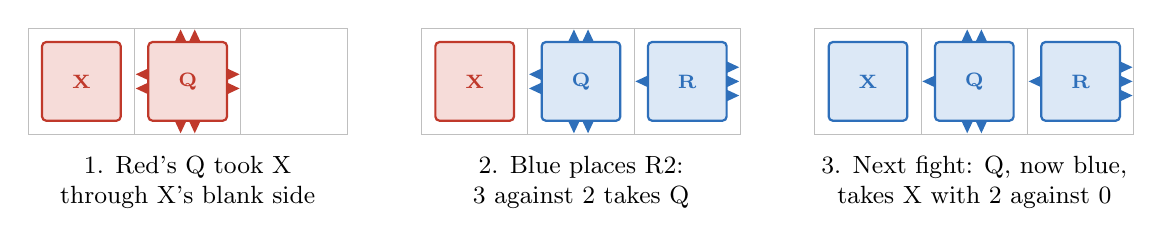
\begin{tikzpicture}[scale=1.35]
  \draw[gray!50, shift={(-0.5,-0.5)}] (0,0) grid (3,1);
  \stone{0}{0}{0}{0}{0}{0}{red}{stoner}{X}
  \stone{1}{0}{2}{2}{2}{2}{red}{stoner}{Q}
  \node[font=\small, align=center] at (1,-0.95) {1. Red's Q took X\\through X's blank side};
  \begin{scope}[xshift=3.7cm]
  \draw[gray!50, shift={(-0.5,-0.5)}] (0,0) grid (3,1);
  \stone{0}{0}{0}{0}{0}{0}{red}{stoner}{X}
  \stone{1}{0}{2}{0}{2}{2}{blue}{stoneb}{Q}
  \stone{2}{0}{0}{3}{0}{1}{blue}{stoneb}{R}
  \node[font=\small, align=center] at (1,-0.95) {2. Blue places R2:\\$3$ against $2$ takes Q};
  \end{scope}
  \begin{scope}[xshift=7.4cm]
  \draw[gray!50, shift={(-0.5,-0.5)}] (0,0) grid (3,1);
  \stone{0}{0}{0}{0}{0}{0}{blue}{stoneb}{X}
  \stone{1}{0}{2}{0}{2}{1}{blue}{stoneb}{Q}
  \stone{2}{0}{0}{3}{0}{1}{blue}{stoneb}{R}
  \node[font=\small, align=center] at (1,-0.95) {3. Next fight: Q, now blue,\\takes X with $2$ against $0$};
  \end{scope}
\end{tikzpicture}
\caption{A chain. X is a blank stone that Red's queen (Q) took in an earlier move. Blue places a level-2 rook (R) to the right of Q. In step 2 two spikes break on each side ($3$ against $2$), Blue keeps $1$ and takes Q. In step 3 Q and X are of different players with Q's spikes between them, so they fight, X turns blue and Q spends one spike.}
\label{fig:chain}
\end{figure}

\begin{figure}[ht]
\centering
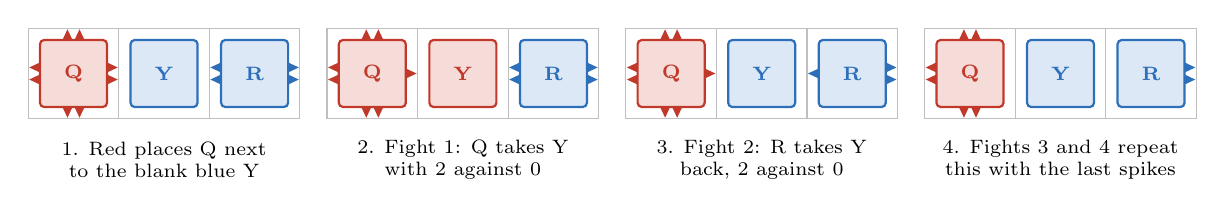
\begin{tikzpicture}[scale=1.15]
  \foreach \px/\cap/\qr/\yc/\yf/\rl in {0/{1. Red places Q next\\to the blank blue Y}/2/blue/stoneb/2, 3.3/{2. Fight 1: Q takes Y\\with $2$ against $0$}/1/red/stoner/2, 6.6/{3. Fight 2: R takes Y\\back, $2$ against $0$}/1/blue/stoneb/1, 9.9/{4. Fights 3 and 4 repeat\\this with the last spikes}/0/blue/stoneb/0}{
    \begin{scope}[xshift=\px cm]
    \draw[gray!50, shift={(-0.5,-0.5)}] (0,0) grid (3,1);
    \stone{0}{0}{2}{\qr}{2}{2}{red}{stoner}{Q}
    \stone{1}{0}{0}{0}{0}{0}{\yc}{\yf}{Y}
    \stone{2}{0}{0}{2}{0}{\rl}{blue}{stoneb}{R}
    \node[font=\scriptsize, align=center] at (1,-0.95) {\cap};
    \end{scope}
  }
\end{tikzpicture}
\caption{A stone reached from two sides. Y is blank. Red's new queen (Q) fights Y first and takes it, then Y is red next to Blue's rook (R) with R's spikes between them, so R takes Y back. Q still has a spike towards Y, so the two lines fight again, until every spike on them is used up and Y stays blue.}
\label{fig:squeeze}
\end{figure}

\paragraph{How the game shows a move.} The game plays a move back as a sequence of fights in the order above: first the new stone's own fights together, then each fight of the chain on its own. Each fight shows the spikes that break off, with nothing drawn over the line. A stone turns over, with the old colour on its front and the new colour on its back, only when it changes colour, so a stone that is taken and taken back in one move turns twice. A golden shield flashes when spikes break on it, a poisonous bite splashes green, a poisoned stone glows and counts down, the Pope hovers on two jet flames until he is grounded, bees fly out of the swarm, Prince Joey crumbles into rubble, and an Old Woman is crowned when she becomes the Grand Empress. Chains of more than twelve fights play faster.

\paragraph{End.} The match ends when the board is full or when a Pope is taken. Each player scores one point per stone of their colour on the full board, and the higher score wins. Taking the Pope wins at once. In the game a drawn match is replayed.

\section{Properties of a move}

\begin{proposition}\label{prop:ends}
Every move ends.
\end{proposition}
\begin{proof}
A fight happens only when at least one of the two facing sides has spikes. Against a golden shield all those spikes break. Otherwise, if one side has more spikes, the winner loses at least one, also a gorilla. If both have the same number, both lose spikes, a gorilla at least one. So every fight removes at least one spike from the board. Spikes are added during a move only when an Old Woman becomes the Grand Empress, which happens at most once for each Old Woman. Poison changes the colour of each poisoned stone at most once. So the number of fights in a move is finite.
\end{proof}

\begin{proposition}\label{prop:clean}
When a move ends, no two stones of the two players touch with a spike between them.
\end{proposition}
\begin{proof}
Step 3 continues as long as such a pair exists. It runs again after every change in step 4, including the promotion of an Old Woman, which is the only event that adds spikes, and the swarm in step 1 only removes spikes. By proposition~\ref{prop:ends} each of these runs ends, so when the move ends no such pair is left.
\end{proof}

In random games with random hands of all pieces and levels, the longest move we saw had $31$ fights.

\begin{proposition}\label{prop:draw}
When the board is full the two scores add up to $16-r$, where $r$ is the number of rubble stones. If $r$ is even, the difference of the scores is even and a draw is possible.
\end{proposition}
\begin{proof}
A placed stone never leaves the board. It changes colour, or it turns into rubble, which scores for nobody. All $16$ squares are filled at the end, so the two scores add up to $16-r$. If Blue scores $b$, the difference is $b-(16-r-b)=2b-16+r$, which is even when $r$ is even. The simulations of section~\ref{sec:balance} contain drawn matches.
\end{proof}

\section{The run}\label{sec:run}

A run is twenty matches. Blue starts with the eight stones P1\^{}, P1>, P1<, N1, B1, R1, Q1, K1: Tiny Tim, Tiny Tony, Tiny Ted, a knight, a bishop, a rook, the queen and the king.

\paragraph{Opponents.} Six regular opponents each play three of the first nineteen matches, plus one extra match for a randomly chosen one, in a random order. The seventh opponent plays match 20. Each regular opponent has three fixed decks: early (matches 1 to 6), middle (7 to 13) and late (14 to 19). Table~\ref{tab:balance} lists all decks. Five regular opponents bring a rare stone in their middle and late decks: Pawnbroker Pete the Gorilla, Sir Neighsalot the Beekeeper, Madame Swerve the Serpent, Lady Lux the Old Woman and Uncle Gambit Prince Joey. The final opponent brings the Pope. Blue places first in odd matches and Red in even matches, and the first player alternates when a drawn match is replayed. The final opponent always places first.

\paragraph{Rewards.} After every won match Blue picks one reward: one of up to three different stones from the hand one level higher, Tiny Tom (P1v) as long as he is not in the hand, or, with probability $1/2$, the rare stone of the opponent just beaten. A stone that joins takes the place of a stone Blue picks. A lost match ends the run. Blue then keeps one stone gained during the run, which replaces the stone in its place in the starting hand of every later run.

\paragraph{Computer player.} Red plays by negamax search with alpha-beta pruning and iterative deepening. Moves are ordered by their immediate gain in points, and stones of equal piece, level and variant are tried once. A position at the search horizon is valued at $100$ times the score difference plus $60$ times the best immediate gain of the side to move, and a taken Pope ends the search with a win or a loss. In its search Prince Joey never collapses. Red searches for $1.0$ seconds per move, the final opponent for $1.6$ seconds. Ties between equally valued moves are broken at random.

\section{Balance by simulation}\label{sec:balance}

\paragraph{Method.} For each phase we fix a reference hand for Blue that stands for a player who took one level after every won match, mostly on the king, the rook, the knight and the bishop, and who gave the queen the place of a pawn after match 13:
\begin{center}
\begin{tabular}{lll}
early & P1\^{} P1> P1v P1< N1 B1\^{} R1 K1 & start \\
middle & P1\^{} P1> P1v P1< N2 B2\^{} R3 K3 & $+6$ levels \\
late & P2\^{} P2> P1v Q1 N4 B3\^{} R4 K4 & $+13$ levels, queen \\
final & P3\^{} P2> P2v Q2 N5 B4\^{} R5 K5 & $+19$ levels, queen \\
\end{tabular}
\end{center}
Both sides are played by the game's own search, fixed at depth $3$ instead of a time limit, so that the strength of both players does not depend on the load of the machine. Each pairing of a reference hand with an opponent deck is played $100$ times with alternating first player and a seeded random generator. Since drawn matches are replayed in the game, the share of wins is counted as wins divided by wins plus losses. A first round with a time limit of $60$ milliseconds per move gave shares that moved by more than $20$ percentage points between repeated runs of $40$ games, which is why the final table uses a fixed depth.

\paragraph{Tuning.} Every deck was tuned automatically. Starting from a hand-made deck, levels are added or removed one at a time, round robin over the stones in the order king, queen, rook, bishop, knight, pawn, and always between $1$ and $5$. A binary search over the number of added or removed levels, with $60$ games per step, picks the number whose share is closest to the target of the phase: $90\%$ for early decks, $75\%$ for middle decks, $55\%$ for late decks and $15\%$ for the final opponent.

\paragraph{Results.} Table~\ref{tab:balance} gives all $19$ pairings. Averaged over the opponents, the reference player wins $91\%$ of early matches, $74\%$ of middle ones, $44\%$ of late ones and $13\%$ against the final opponent. These shares come from fresh games and differ from the $60$-game estimates of the tuning. Taking the shares as independent and averaging over random orders of the opponents, the reference player clears a whole run with probability $5.5\times10^{-5}$, about once in $18{,}000$ runs. Kept stones raise this for later runs.

\begin{table}[ht]
\centering
\small
\begin{tabular}{llcrrrr}
\toprule
opponent & phase & deck & won & lost & drawn & share \\
\midrule
Pawnbroker Pete & early & P1\^{} P1> P1v P1< P1\^{} P1> N1 K1 & 99 & 0 & 1 & 100\% \\
 & middle & P3\^{} P3> P3v P3< P3\^{} N3 N3 K3 & 86 & 5 & 9 & 95\% \\
 & late & P3\^{} P3> P3v N4 N3 N3 Q3 K4 & 49 & 33 & 18 & 60\% \\
\addlinespace
Sir Neighsalot & early & N1 N1 P1\^{} P1> P1v P1< P1\^{} K1 & 97 & 0 & 3 & 100\% \\
 & middle & N3 N3 N3 N3 P3\^{} P2> R2 K3 & 78 & 7 & 15 & 92\% \\
 & late & N3 N3 N3 N3 Q3 P3\^{} R3 K4 & 42 & 32 & 26 & 57\% \\
\addlinespace
Madame Swerve & early & B1\^{} B1> P1\^{} P1> P1v P1< P1\^{} K1 & 87 & 5 & 8 & 95\% \\
 & middle & B3\^{} B3> B3v P2\^{} P1> P1v N1 K3 & 40 & 42 & 18 & 49\% \\
 & late & B3\^{} B3> B3v B3< Q3 P2\^{} N3 K4 & 45 & 37 & 18 & 55\% \\
\addlinespace
Blocky Barb & early & R1 P1\^{} P1> P1v P1< P1\^{} P1> K1 & 62 & 20 & 18 & 76\% \\
 & middle & R2 R2 R1 P2\^{} P1> P1v N2 K3 & 77 & 7 & 16 & 92\% \\
 & late & R3 R3 R3 Q3 P2\^{} P2> N3 K4 & 12 & 65 & 23 & 16\% \\
\addlinespace
Lady Lux & early & B2\^{} B2> P2\^{} P2> P2v P2< P1\^{} P1> & 80 & 12 & 8 & 87\% \\
 & middle & B3\^{} B3> B3v P1\^{} P1> P1v N1 K3 & 41 & 45 & 14 & 48\% \\
 & late & Q3 Q2 Q2 P2\^{} P2> N2 B3\^{} K2 & 30 & 52 & 18 & 37\% \\
\addlinespace
Uncle Gambit & early & N1 B1\^{} R1 P1\^{} P1> P1v P1< P1\^{} & 71 & 10 & 19 & 88\% \\
 & middle & N2 B2\^{} R3 R1 P2\^{} P1> P1v P1< & 57 & 24 & 19 & 70\% \\
 & late & N3 B3\^{} R3 Q3 Q2 P2\^{} P2> K2 & 37 & 51 & 12 & 42\% \\
\addlinespace
The Obsidian Monarch & final & Q4 Q4 R4 B3\^{} N3 N3 K5 P3\^{} & 11 & 71 & 18 & 13\% \\
\bottomrule
\end{tabular}
\caption{The reference player against every opponent deck, $100$ games each at search depth $3$. The share is won divided by won plus lost.}
\label{tab:balance}
\end{table}

\paragraph{Steps of one level.} A single level can move the share far, so the tuning cannot always land on its target, and its $60$-game estimates differ from the $100$-game results of table~\ref{tab:balance}. For Pawnbroker Pete's middle deck the search ended at $8$ added levels with $96\%$ in its $60$ games, and the $100$-game check gives $95\%$. A pawn has a single spiked side, so a level adds only one spike to it, while a level on a rook or a queen adds four.

\section{Conclusion}

Chain Stones in its current form is a four-sided placement game with the six chess pieces, levels, and fights that continue until no two stones of different colours touch across a spike. Every move ends because every fight uses up a spike, and the score difference at the end is even. The twenty-match run was balanced with simulated games at a fixed search depth. For a player who takes a level after every win, the share of won matches falls from $91\%$ in the early phase to $13\%$ against the final opponent. Two questions remain open: the exact value of the $4\times4$ game for given hands, and how far a human player's results differ from those of the depth-3 reference player.

\paragraph{Related games.} Chain Stones belongs to the same family as Triple Triad, the card game from \emph{Final Fantasy VIII}, which is played on a $3\times3$ board with tiles that capture weaker neighbours. The breaking spikes, the capture in both directions, the chains that spread outwards and the run of matches against fixed hidden decks are specific to Chain Stones.

\paragraph{Reproducibility.} The rules engine and computer player (\texttt{balance/core.js}, identical to the engine in the game), the simulator (\texttt{balance/simd.js}), the tuning search (\texttt{balance/tune.mjs}), the script that reads the decks from the game and runs every pairing (\texttt{balance/table.mjs}) and the results of table~\ref{tab:balance} (\texttt{balance/results.json}) are included with this paper.

\appendix
\section{The first version on the $3\times3$ board}

The first version of the game had no pieces, levels or chains. Each stone had $0$ to $3$ spikes per side, dealt at random so that both hands had the same total strength and differed only in shape. A taken stone did not start further fights. On the $3\times3$ board Blue placed five stones and Red four.

That version was solved exactly with a C solver (negamax, alpha-beta pruning and a transposition table) for $9{,}000$ random deals. Under perfect play the first player won $64.7\%$ of deals ($95\%$ confidence interval $63.7\%$ to $65.7\%$). Draws were impossible there, since the nine stones always split as $b+r=9$ and the difference $9-2r$ is odd. Table~\ref{tab:values} gives the distribution of values. Some corner opening was optimal in $95.2\%$ of $500$ fully analysed deals, and in a typical won deal $91\%$ of all openings lost. Among hands of equal total strength, the hand with more blank sides won more often, from $30\%$ to $93\%$ as the difference in blank sides went from $-4$ to $+4$. The solver and its data are in \texttt{solver/}, and the full write-up of that version is \texttt{chain\_stones\_v1.pdf}.

\begin{table}[ht]
\centering
\begin{tabular}{lrrrrr}
\toprule
value (Blue $-$ Red) & $-3$ & $-1$ & $+1$ & $+3$ & $+5$ \\
\midrule
deals & 26 & 3{,}148 & 5{,}407 & 414 & 5 \\
share & 0.3\% & 35.0\% & 60.1\% & 4.6\% & 0.1\% \\
\bottomrule
\end{tabular}
\caption{First version: exact values of $9{,}000$ random $3\times3$ deals.}
\label{tab:values}
\end{table}

\end{document}
